\begin{figure}[t!]
\centering
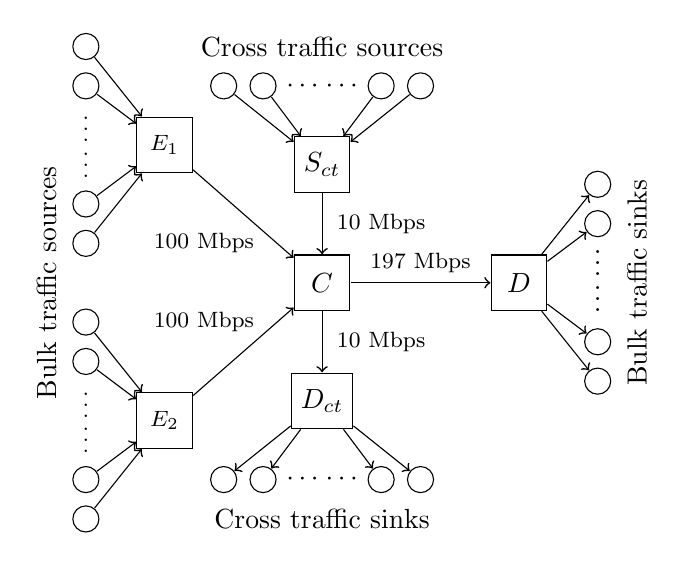
\begin{tikzpicture}
\pgfmathsetmacro{\Rsize}{20}
\pgfmathsetmacro{\Csize}{2}
\tikzset{
line width=0.6pt
}
\node[rectangle,draw=black,minimum size=\Rsize] (E1) at (1.5, 0.5*8.5) {\footnotesize $E_1$};
\foreach \i in {6,7,10,11}
{
 \node[circle,draw=black,minimum size=\Csize] (\i) at (0.5,0.5*\i) {};
 \draw[->] (\i) -- (E1);
}
\node (xs1) at (0.5, 0.5*8.5 - 0.15) {\footnotesize $\vdots$};
\node (xs2) at (0.5, 0.5*9.0 + 0.05) {\footnotesize $\vdots$};

 \node[rectangle,draw=black,minimum size=\Rsize] (E2) at (1.5,0.5*2.5-0.5) {\footnotesize $E_2$};
\foreach \i in {1,2,5,6}
{
 \node[circle,draw=black,minimum size=\Csize] (\i) at (0.5,0.5*\i-1.0) {};
 \draw[->] (\i) -- (E2);
}
\node (xs1) at (0.5, 0.5*1.5 - 0.15) {\footnotesize $\vdots$};
\node (xs2) at (0.5, 0.5*2.0 + 0.05) {\footnotesize $\vdots$};


\node (e1cap) at (2.0, 0.5*4.0) {\footnotesize $100$ Mbps};
\node (e2cap) at (2.0, 0.5*6.0) {\footnotesize $100$ Mbps};
\node (corecap) at (4.75, 0.5*5.5) {\footnotesize $197$ Mbps};
\node (crosscapsource) at (4.25, 0.5*3.5) {\footnotesize $10$ Mbps}; 
\node (crosscapsink) at   (4.25, 0.5*6.5) {\footnotesize $10$ Mbps};


\node[rectangle,draw=black,minimum size=\Rsize] (C) at (3.5, 0.5*5) {$C$};
\draw[->] (E1) -- (C);
\draw[->] (E2) -- (C);

\node[rectangle,draw=black,minimum size=\Rsize] (CT1) at (3.5, 0.5*8) {$S_{ct}$};
\draw[->] (CT1) -- (C);
\foreach \i in {1,2,5,6}
{
 \node[circle,draw=black,minimum size=\Csize] (CS\i) at (0.5*\i+1.75, 0.5*8+1.0) {};
 \draw[->] (CS\i) -- (CT1);
}
\node (y1) at (3.25, 0.5*8+1.0) {$\cdots$};
\node (y3) at (3.75, 0.5*8+1.0) {$\cdots$};


\node[rectangle,draw=black,minimum size=\Rsize] (D) at (6.0, 0.5*5) {$D$};
\draw[->] (C) -- (D);

\foreach \i in {2,3,6,7}
{
 \node[circle,draw=black,minimum size=\Csize] (d\i) at (7.0,0.5*\i+0.25) {};
 \draw[->] (D) -- (d\i);
}
\node (x1) at (7.0, 0.5*6.0 - 0.15) {$\vdots$};
\node (x3) at (7.0, 0.5*4.5 + 0.15) {$\vdots$};

\node[rectangle,draw=black,minimum size=\Rsize] (CD1) at (3.5, 0.5*2.0) {$D_{ct}$};
\draw[->] (C) -- (CD1);
\foreach \i in {2,3,6,7}
{
 \node[circle,draw=black,minimum size=\Csize] (ctds\i) at (1.25 + 0.5*\i,0) {};
 \draw[->] (CD1) -- (ctds\i);
}
\node (y1) at (3.25, 0) {$\cdots$};
\node (y3) at (3.75, 0) {$\cdots$};
\node[rotate=90] (tbulk1) at (0, 2.5) {{Bulk traffic sources}};

\node[rotate=90] (tbulk2) at (7.5, 2.5) {{Bulk traffic sinks}};

\node (tct1) at (3.5, 5.5) {{Cross traffic  sources}};

\node (tcts) at (3.5,-0.5) {{Cross traffic sinks}};

\end{tikzpicture}
\caption{ The network topology used for packet-level simulations. 
The bulk of the traffic passes through two distinct edge routers which then merge at a common core router.
The topology also consists of cross traffic comprising of both long and short-lived flows. }
\label{fig:crosstraffic}
\end{figure}